\documentclass[a4paper, 12pt,oneside]{article} 
%\documentclass[a4paper, 12pt,oneside,draft]{article} 
\usepackage{preamble}
%--------------------- ACTUAL FILE ---------------------- %
\begin{document} 
%%%
	\begin{titlepage}
    \newcommand{\HRule}{\rule{\linewidth}{0.5mm}} % Defines a new command for the horizontal lines, change thickness here
    
    \center  % Center everything on the page
     
    %----------------------------------------------------------------------------------------
    %   HEADING SECTIONS
    %----------------------------------------------------------------------------------------

    \vspace{3cm}
    \textsc{\LARGE École polytechnique fédérale de Lausanne}\\[1.5cm] % Name of your university/college
    
    \textsc{\Large Regression Methods Project Report}\\[0.5cm] % Major heading such as course name
    \textsc{\large Coin-Data Regression Study}\\[0.5cm] % Minor heading such as course title
    
    %----------------------------------------------------------------------------------------
    %   TITLE SECTION
    %----------------------------------------------------------------------------------------
    
    \HRule \\[0.4cm] % line above and under the title
    
    
    % Title of your document
    
    \HRule \\[1.5cm]
     
    %----------------------------------------------------------------------------------------
    %   AUTHOR SECTION
    %----------------------------------------------------------------------------------------
    
    \begin{minipage}{0.4\textwidth}
    \begin{flushleft} \large
    
    \emph{Authors:}\\
    Tara \textsc{Fjellman}\\
    Rayan \textsc{Harfouche}\\
    
    
    
    
    \end{flushleft}
    \end{minipage}
    ~
    \begin{minipage}{0.4\textwidth}
    \begin{flushright} \large
    
    \emph{Professor:} \\
    Anthony \textsc{Davison}\\
    \end{flushright}
    \end{minipage}\\[10cm]
    %
    
    
    %----------------------------------------------------------------------------------------
    %   LOGO SECTION
    %----------------------------------------------------------------------------------------
    
    
\includegraphics[width=0.4\linewidth]{Logo-1 .pdf}\\[1cm] 
    % Include a department/university logo - this will require the graphicx package
     
    %----------------------------------------------------------------------------------------
    
    \vfill % Fill the rest of the page with whitespace
    
    \end{titlepage} 
	% Add titlepage
	\clearpage
	\tableofcontents
	\thispagestyle{empty}
	\vspace{2cm}
	\section*{Abstract}
		context of the original paper (with their claims). The paper that won the 2024 IgNobel Prize in Probability took a Bayesian approach to studying the statistics behind the coin-flipping process. Its main goal was to confirm a prediction made by a physical model of human coin tossing developed by Diaconis, Holmes, and Montgomery (DHM; 2007); i.e. that when people flip an ordinary coin, the probability of it landing on the same side it started is about 51\%. 
		It also revealed considerable between-people variation in the degree of this same-side bias, as well as its decrease as more coins were flipped. 

		The goal of this report is two fold. On the one side, we aim to investigate similar questions with a regression approach : 
		is there evidence for between-person, between-coin, or even person-coin pair differences ? To what extent does flipping experience affect the observed same-side bias ?
		In addition, we also investigate the differences between GLM and WLS approaches; as well as muscle memory effects (through outcomes of recent flips). 
	\clearpage
	\pagenumbering{arabic}
	\setcounter{page}{1}
	\section{Introduction}
		Before diving into the analysis, we provide a brief overview of the datasets main features and the models we consider. Our exploratory analysis is available as a Jupyter notebook, and provides more detail. 

		The dataset is composed of throws from 48 people using 44 coins in total. Given the study did not impose strict guidelines for coins to be used, the design is heavily unbalanced. Eighteen coins have only been thrown by a single person, while some of them have been thrown by more than 20 people. Also, more than half the people have only flipped 5 or less different coins, while someone threw 11 different ones. As for the the person-coin pairs, most have fewer or equal to 1000 throws, while some have around 10000 ones. This severe unbalance must be kept in mind during the study, given it can pose challenges during model interpretation. 

		After plotting the same-side rates across people, coin and person-coin combinations, we deemed it relevant to investigate models considering both person and coin as covariates, as well as individual person-coin pairs. Following the advice given on the project statement, we also branched our analysis in Binomial-response GLM and WLS approaches. 

		Motivated by impacts of muscle-memory on the flipping, we additionally investigated aspects such as time-varying same-side rates and memory between successive throws.
	\section{Analysis}
		\subsection{Model Comparison}
			In this section, we introduce and compare different models for the same-side rate. 

			Before thinking about models, we thought about whether transforming the response was needed. Given the same-side rates where clustered around 50\% with few changes by at most factors of locally 0.66 and 1.5, we did not see any reason a priori to apply a transformation to the response.
			
			As for the covariates we considered in our models, we of course included the person throwing and the coin being thrown as categorical covariates. Due to the mention in the original paper of the existence of learning effects, and the potential we saw in these to alias with coin effects (see discussion in [ref section]), we also wanted to include time dependence in the dataset. This was done by considering the version of the data that is composed of ordered sequences of 100 (or so) throws at a time. Considering this data also allowed us to try and consider effects of coins nested within people, trying to capture subjectivity in how people perceive given coins. Indeed, doing this on the averaged data would have yielded a saturated model. 
			%\begin{itemize}
			%	\item \texttt{1}, corresponding to a constant model.
			%	\item \texttt{1+C(person)}, corresponding to a model with the person as a covariate.
			%	\item \texttt{1+C(person)+C(coin)}, corresponding to a model with the person and the coin as covariates.
			%	\item \texttt{1+C(person)+C(coin)+C(person):C(coin)}, corresponding to a model with the person, the coin, and the interaction between the person and the coin as covariates.
			%\end{itemize}
			%* model 4 could seem redundant due to nesting-main effect, but we ....
			
			[explain why eliminated some covariates ...??]

			In the next section, we start by introducing the theory on which we base our model selection. 
			\subsubsection{Tools For Selection}
				Following the suggestion in the project statement, we compare candidate models both with help of Akaike's Information Criterion (AIC) and Likelihood Ratio Tests (LRTs). 

				We recall that AIC is defined as 
				\begin{gather}
					\text{AIC}:=2p-2\ln(\hat L),
				\end{gather}
				with $p$ the number of degreas of freedom of the model and $\hat L$ the value of the maximised likelihood function for the model. By minimising AIC over candidate models, one is therefore rewarding model fit, while penalising by a $2p$ term to counter overfitting. Its goal is therefore to yield parsimonious predictive models. It does not make any assumption about models being of similar interpretation or nested. 

				In contrast, LRT is specifically designed for comparing a model $A$ with a nested (or restricted) one $B$. It is based on the fact that 
				\begin{gather}
					\lambda_{LR}=-2\ln\left[\frac{\sup_{\theta\in\Theta_B}\mathcal{L(\theta)}}{\sup_{\theta\in\Theta_A}\mathcal{L(\theta)}}\right]
					\overset{H_0}{\sim} \chi^2_{p_A-p_B},
				\end{gather}
				where $\Theta_A\supset\Theta_B$ respectively are the parameters spaces (of dimension $p_a>p_b$) associated to models $A$ and $B$, and $H_0$ is the null hypothesis : $\theta^*\in\Theta_B$. Given this definition, LRTs are used to shed light on whether extra degrees of freedom improve the model significantly better than chance. This has applications in explanatory models, but might be of limited use in the context of model selection due to being prone to overfitting. This is particularly true when testing many models, as tests become correlated and give rise to spurious results [cite davison slides ?].

				[MAYBE MENTION DEVIANCE??]
			\subsubsection{Diagnostic Plots}
				In this report, the diagnostics we decided to include where 
				\begin{itemize}
					\item A QQ plot to check normality of normalised residuals. Pearson studentized residuals were used for WLS models while the presented $r^*$ were used for GLM models. Normality corresponds to a roughly straight line, while outliers, skewness and heavy tails are easily spotted as deviations from it.
					\item A scatter plot of residuals as a function of fitted values, to assess linearity and homoscedasticity. [TO FILL] were used for WLS models, while deviance residuals where used for GLM models. Linearity corresponds to residuals that stay centred around 0 across the fitted values, while homoscedasticity corresponds to errors whose spread is constant across the fitted values.
					\item Cook's distance as a function of data index to reveal highly influential data points. Points over the $8/(n-2p)$ threshold are given a closer look (in order of importance). 
					\item Scatter plots (resp. box plots for categorical covariates) of residuals as a function of the covariates of interest. These are used to check for independence between residuals and the covariates. If there is independence, the residuals look uncorrelated to the covariates. 
				\end{itemize}
				This decision was motivated by our understanding of section 1.4 about diagnostics found in [CITE DAVISON SLIDES]. 
			\subsubsection{WLS Approach}
			In this section, we consider the normal approximation for the binomial variable $R$ with denominator $m$. Having that the success probability is fairly close to 0.5 we get $p(1-p)$ approximately equal to 1/4. Hence we end up with: $R/m \sim N(p,1/(4m))$. 

			We then make a linear fit using weighted least squares, where  weight associated to each entry is proportional to the inverse of the variance, that only depending on $m$.

			We consider different models, starting with a constant model, then adding in the following order the 

			\begin{table}[htb]
				\centering
				\caption{Model comparison based on AIC values.}
				\label{tab:model-comparison}
				\begin{tabular}{lc}
				\toprule
				Model Formula (RHS) & AIC \\
				\midrule
				1 & 159.76 \\
				1 + C(person) & 12.89 \\
				1 + C(person) + agg & 0.00 \\
				1 + C(person) + agg + C(coin) & 29.21 \\
				1 + C(person) + agg + C(person):C(coin) & 123.98 \\
				\bottomrule
				\end{tabular}
			\end{table}

			Table of comparison of the models using the likelihood ratio tests. 

			\begin{table}[htb]
				\caption{LRTs table}
				\label{tab:LRT-model-comparison}
				\begin{tabular}{lcc}
				\toprule
				Tested model & Restricted Model & p-value \\
				\midrule
				1 + C(person) & 1 & 0.00 \\
				1 + C(person) + agg & 1 + C(person) & 0.00 \\
				1 + C(person) + agg + C(coin) & 1 + C(person) + agg & 0.09 \\
				1 + C(person) + agg + C(person):C(coin) & 1 + C(person) + agg & 0.02 \\
				\bottomrule
				\end{tabular}
				\end{table}

			\subsubsection{GLM Approach}
			In this section, instead of relying on an approximation to fit a Least Squares models, we take into account the nature of the data by using a GLM. Indeed, given the binomial nature of aggregated data, using a binomial-response GLM seems natural. 
			\begin{table}[htb]
				\centering
				\caption{Model comparison for different models.}
				\label{tab:model-comparison}
				\begin{tabular}{lccc}
				\toprule
				Model & Deviance & AIC & Model DF \\
				\midrule
				\texttt{1} & 3942.13 & 187.84 & 0 \\
				\texttt{1+person} & 3676.20 & 13.91 & 46 \\
				\texttt{1+person+agg} & 3660.29 & 0.00 & 47 \\
				\texttt{1+person+agg+coin} & 3602.26 & 25.97 & 89 \\
				\bottomrule
				\end{tabular}
			\end{table}
			More specifically, we consider a Logit link as it leads to easily interpretable results, meaning we model $\mathbb{E}[y\mid x]=\exp\left(\sum_i \beta_i x_i\right)$ with binomial errors. We expect this to lead to more accurate results than the WLS approximation, especially for entries having $R/M\not\approx 1/2$.
			\begin{table}[htb]
				\centering
				\caption{Likelihood ratio tests between models.}
				\label{tab:llr-comparison}
				\begin{tabular}{llc}
				\toprule
				Tested model & Restricted model & $p$-value \\
				\midrule
				\texttt{1+person} & \texttt{1} & 0.00e+00 \\
				\texttt{1+person+agg} & \texttt{1+person} & 6.63e-05 \\
				\texttt{1+person+agg+coin} & \texttt{1+person+agg} & 5.09e-02 \\
				\bottomrule
				\end{tabular}
			\end{table}
			As for the considered covariates, we follow what is done for the WLS approach. The only difference being in the interpretation of the coefficients and the in the fact that we omit the model with coins nested within people. Indeed, even the \texttt{0+person:coin} model did not give any signs of convergence after 100 IRLS iterations. We tried fitting it with BFGS, but did not succeed either as the hessian resulted to be non-full rank. The analysis of deviance and LRT tables for the models that converged are \ref{tab:model-comparison} and \ref{tab:llr-comparison}.
			\begin{figure}[htb]
				\centering
				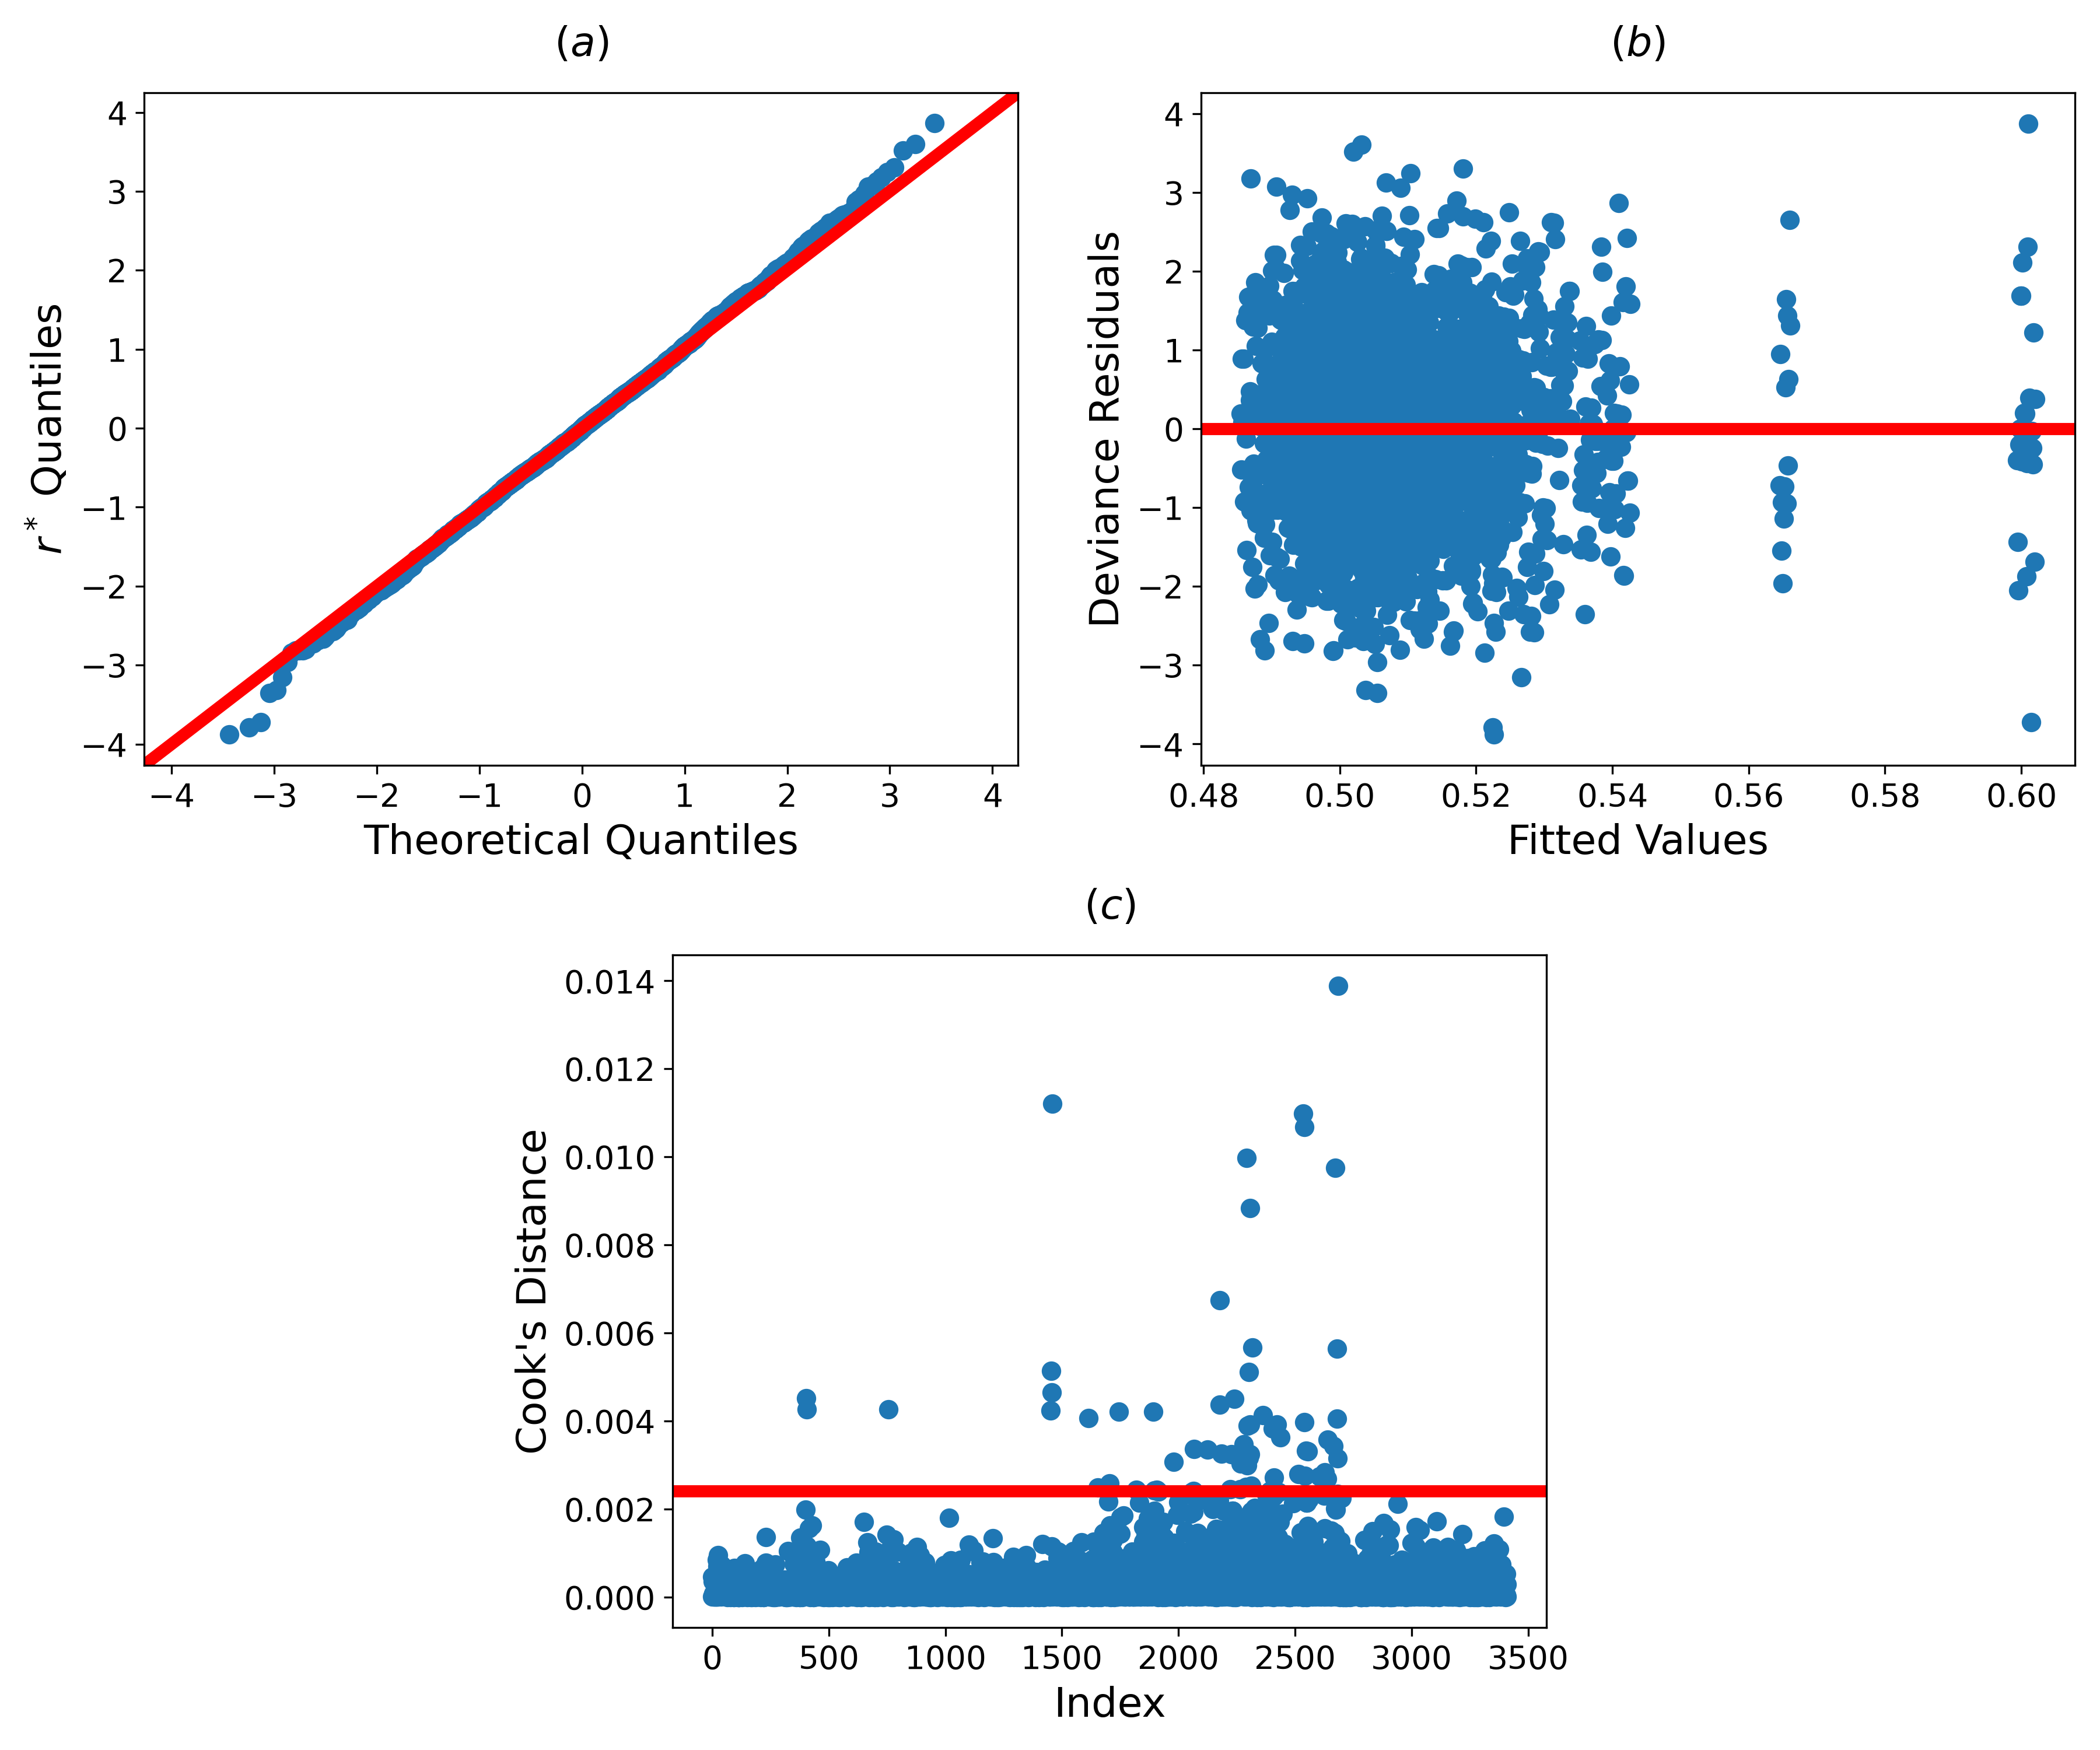
\includegraphics[width=0.85\textwidth]{GLM_diagnostics.png}
				\caption{Diagnostics for the selected GLM model. (a).}
				\label{fig:glm-diagnostic}
			\end{figure}
			The diagnostic plots for the \texttt{1+person+agg+coin} model are in \ref{fig:glm-diagnostic} and \ref{fig:dev-resid-vs-covariates}. 
			\begin{figure}[htb]
				\centering
				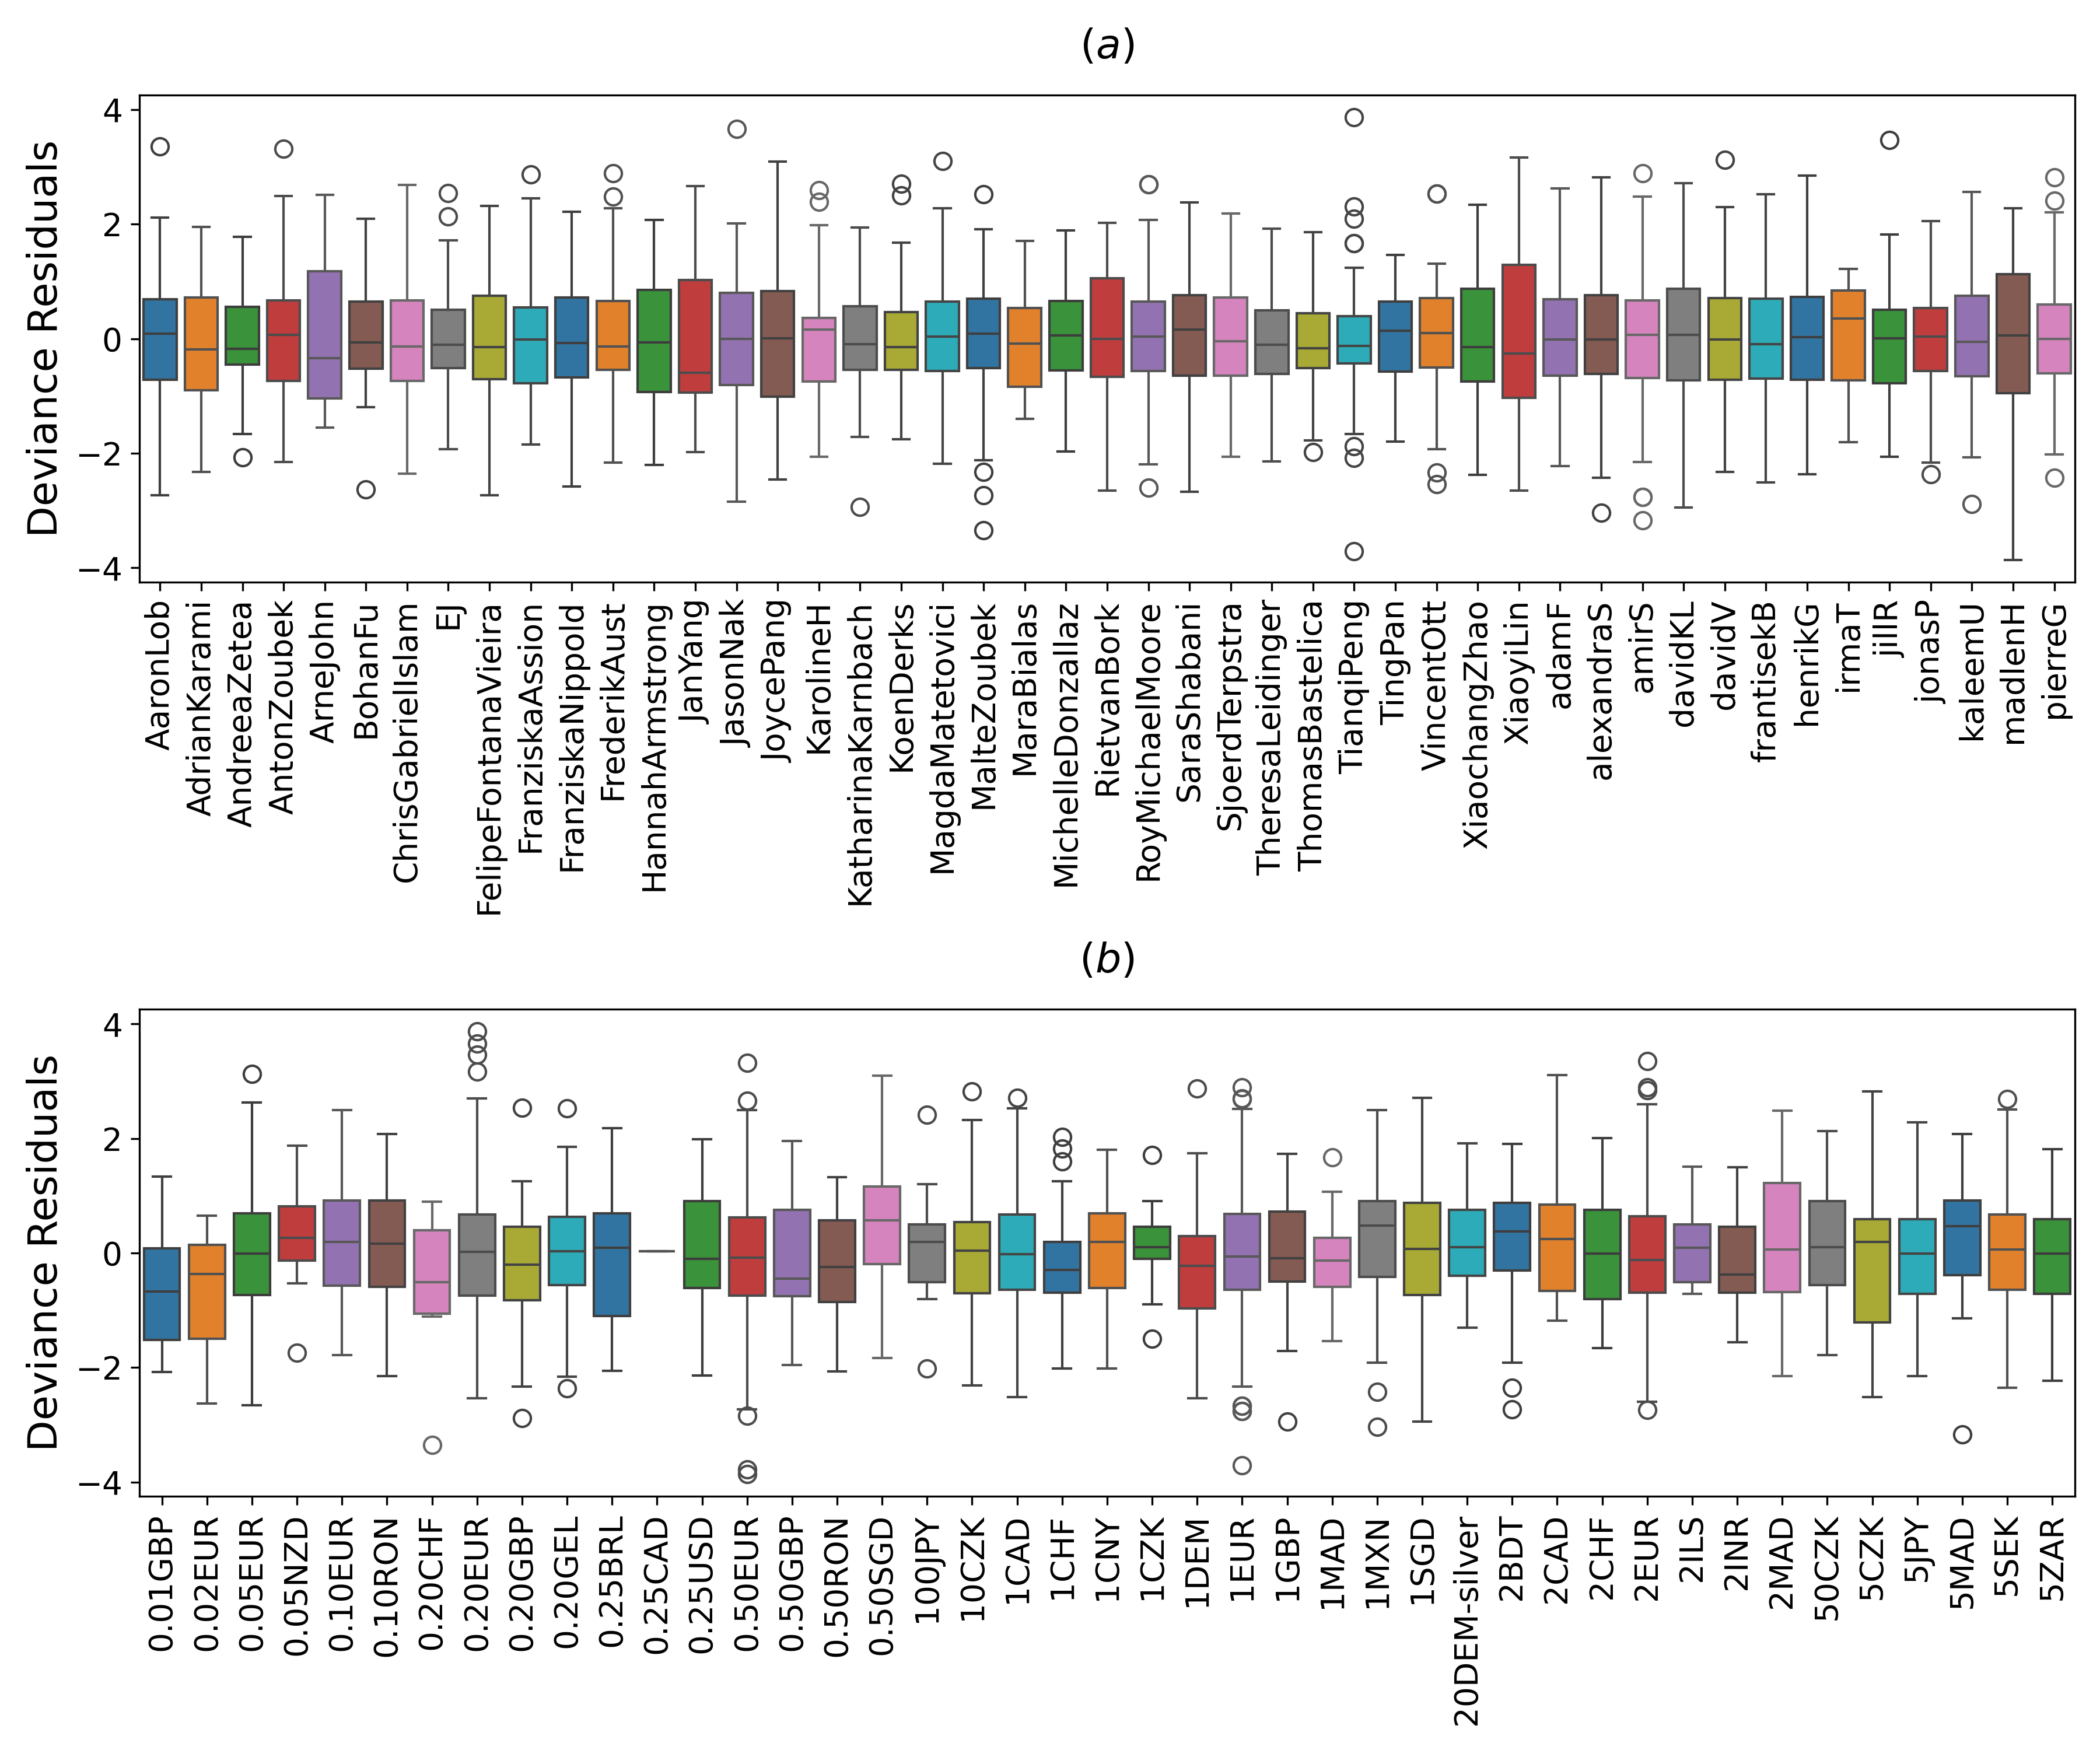
\includegraphics[width=0.95\textwidth]{dev_resid_vs_covariates.png}
				\caption{Dev-resid as a function of (a) person and (b) coin.}
				\label{fig:dev-resid-vs-covariates}
			\end{figure}	
		\subsection{Unusual Observations}

		\subsection{Zoom on Learning Effects}
			We now give a closer look at the learning effects associated to the \texttt{agg} term in the model. We do this by representing the observed and predicted person-averaged same-side rate as a function of the number of throws.  Note that the confidence interval on the prediction was derived in Monte Carlo fashion as the variance between people was found to be larger than that resulting from the uncertainty on the estimated coefficients. 
			The corresponding figure is \ref{fig:learning-effects}. 
			\begin{figure}[htb]
				\centering
				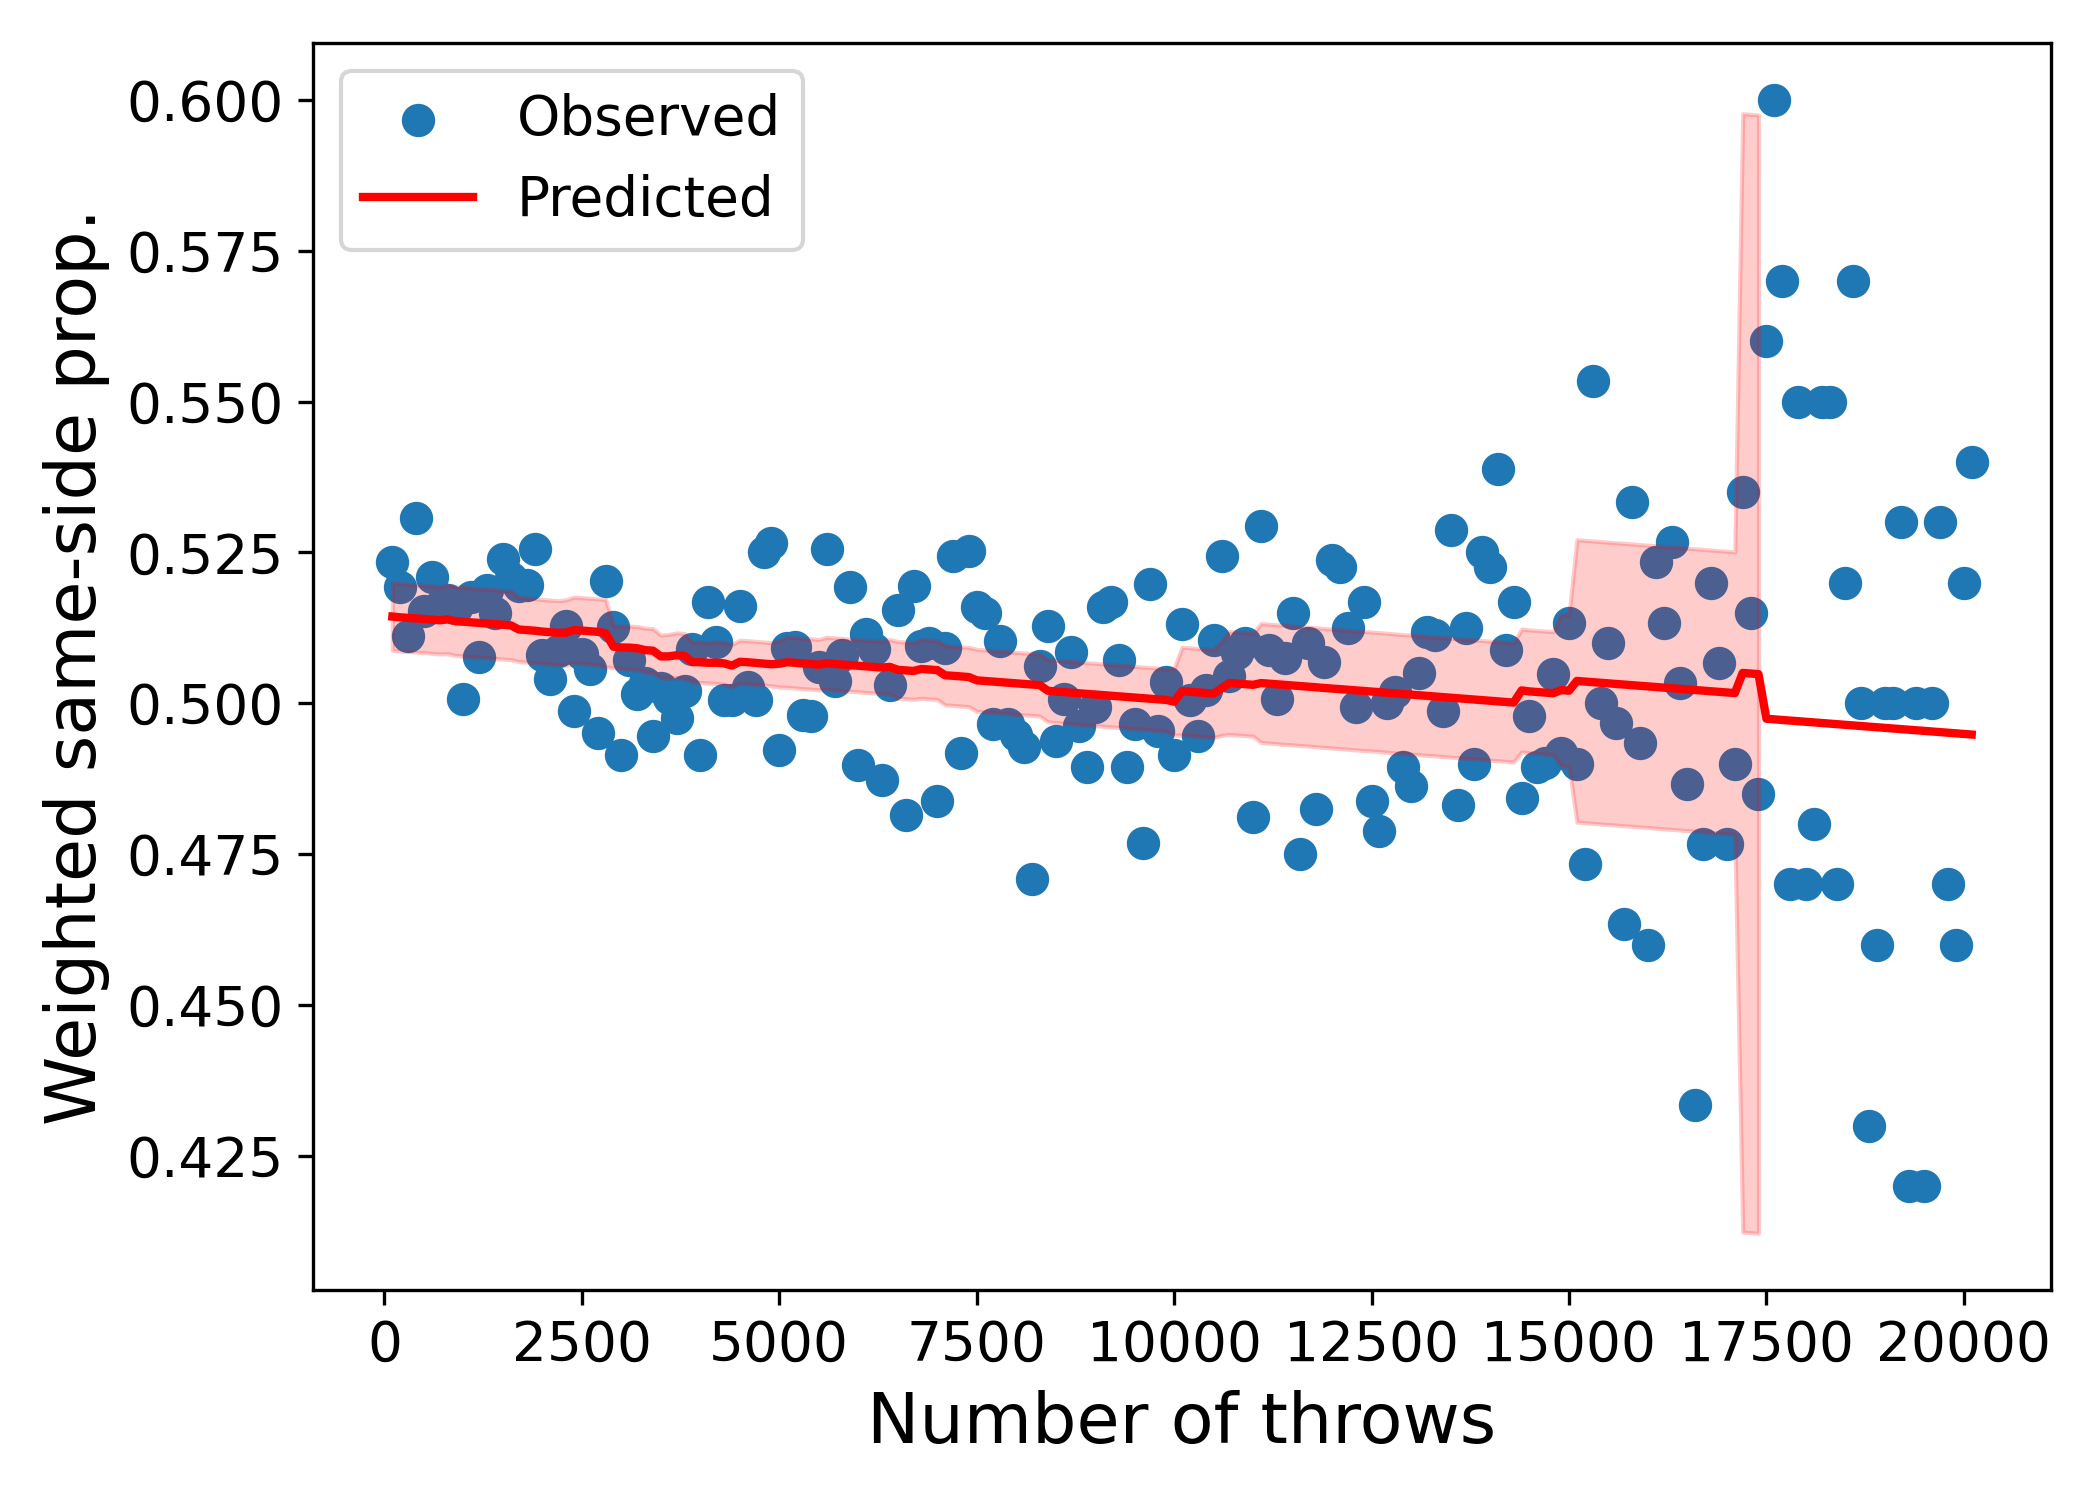
\includegraphics[width=0.5\textwidth]{learning_effects.png}
				\caption{Learning effects.}
				\label{fig:learning-effects}
			\end{figure}
		\subsection{Memory Effects}
		In this section we shift our focus to memory effects. We do so motivated by the fact that we deem it probable a priori that successive throws are more similar to each other than randomly selected ones. Indeed, one could imagine that after two same-side throws, the next could end being a same-side one two with a probability higher than the base rate. 
		
		To test this we start by considering the data consisting of individual throw outcomes. To this, we add columns corresponding to 
		\begin{itemize}
			\item same-side indicator variables,
			\item same-side indicator variables for the penultimate throw,
			\item same-side indicator variables for the antepenultimate throw.
		\end{itemize}
		To deal with the boundary effects between sequences of flips, we removed the two first entries of each sequence. 
		%To speed up the computations
		
		We then define the constant model \texttt{1}, the model including memory about the penultimate throw \texttt{1+hop1\_mem}, and the one including memory about the two previous throws \texttt{1+hop1\_mem+hop2\_mem}. The analysis of deviance associated to these models is found in \ref{tab:memory-model-comparison}. Given the uni-directionality of these results, no further analysis was made.  
		\begin{table}[htb]
			\centering
			\caption{Model comparison for models including : no memory, 1-hop memory and 2-hop memory.}
			\label{tab:memory-model-comparison}
			\begin{tabular}{lccc}
			\toprule
			Model & Deviance & AIC & Model DF \\
			\midrule
			\texttt{1} & 474381.54 & 0.00 & 0 \\
			\texttt{1+hop1\_mem} & 474380.73 & 1.19 & 1 \\
			\texttt{1+hop1\_mem+hop2\_mem} & 474380.53 & 2.98 & 2 \\
			\bottomrule
			\end{tabular}
		\end{table}
	\section{Discussion}
		\subsection{Model Comparison}
		\subsubsection{WLS Approach}
		\subsubsection{GLM Approach}
			We first consider the model comparison tables \ref{tab:model-comparison} and \ref{tab:llr-comparison}. 
			Upon inspection of these, we see that the evidence for between-person variations is extremely strong. The deviance decreases by more than 5.5 points per degree of freedom on average, and the AIC drops by more than 170. Similarly, there is overwhelming evidence for time-dependence in the same-side bias. By itself, the term for example yields a deviance decrease of 15. A closer look at this contribution is given in the \ref{sec:disc-learning-effects}. When it comes to between-coin differences, the evidence is nowhere near as strong. Indeed, AIC increases by around 25 when compared to the \texttt{1+person+agg} model, reflecting clear overfitting. The associated LRT is around .05, meaning coin-effects might still help in explaining part of the deviance. A better evaluation of this could probably be obtained by considering a smaller scale, balanced-design study. Indeed, in the considered dataset, coin and time effects where aliased\footnote{Adding \texttt{coin} to the \texttt{1+person} model explained around 10 units of deviance more than when it was added in the \texttt{1+person+agg} model.}. This was a result of there being a strong time effect on same-side bias, and some coins being flipped many more times than others. 
			Given these elements, one would definitely prefer the \texttt{1+person+agg} model for prediction purposes.  

			We now move to analysing the diagnostics of the selected model. Looking at (a) and (b) of \ref{fig:glm-diagnostic}, we see that the residuals are for the most part appropriately normal and homoschedastic. Slight anomalies are observed in the QQ plot for the largest and smallest residuals, as well as for the residuals associated to the largest fitted same-side rate. Looking up the entries associated to the largest Cooks distances, we notice these are associated to sequences of throws where [TO FILL]
			\begin{itemize}
				\item best model (AIC vs LRT) + interpretation of significance (wobble )
				\item discussion of diagnostics 
				\item (rational of including agg, presentation of used residuals with assumptions)
				\item 
				\item comparison with WLS (coefs ?? accuracy ?)
			\end{itemize}

		\subsection{Unusual Observations}

		\subsection{Zoom on Learning Effects}\label{sec:disc-learning-effects}
			Analysing \ref{fig:learning-effects}, we see that the averaged same-side rate seems to start at a value around 51\%, and then decreases to reach values closer to 50\%. The observed uncertainty/spread can however no be neglected, given the limited number of people involved in the study. 
			
			This would be consistent with the fact that the physical model [CITATION NEEDED] predicts a same-side bias due to the ``wobble'' in people's throws. Indeed, we can imagine that with practice, participants progressively reduce the amount of ``wobble'', until they reach perfect throw, for which there is no bias. 

			As for the type of dependence, the simple linear term at the exponential seems to provide a good fit.  
		\subsection{Memory Effects}
		Looking at \ref{tab:memory-model-comparison}, we see there is no support in favour of memory effects relative to the constant model. The deviance decreases by around .8 due to the introduction of the penultimate throw memory and only a further .2 when including memory of the antepenultimate throw. Another factor that shows this is the increase by $>$1 and $\approx 3$ respectively in AIC compared to the constant model.
		The fact that memory about antepenultimate outcome seems to matter even less than memory about the penultimate outcome does make nonetheless intuitive sense. 

		This (non-) finding can in itself be regarded as reassuring in a way. Specifically, it might contribute to rule out concerns of the authors of the original paper regarding the potential same-side bias induced by participants knowing about the goal of the study. Indeed it seems far-fetched that someone could bias their throws without relying on muscle memory. 
	\section{Conclusion}
	\section*{Acknowledgements}
	\section*{References}
		\noindent[1] F. Bartoš et al., `Fair coins tend to land on the same side they started: Evidence from 350,757 flips', Jun. 02, 2024, arXiv: arXiv:2310.04153. doi: 10.48550/arXiv.2310.04153.
		\newline[2] Anthony Davison, `Regression Methods'. Accessed: Jan. 07, 2025. [Online]. Available: \url{https://moodle.epfl.ch/pluginfile.php/3309119/mod_resource/content/6/RMNotes.pdf}
		\newline[3] nzcoops, `Anova - Type I/II/III SS explained - R-bloggers'. Accessed: Jan. 07, 2025. [Online]. Available: \newline\url{https://www.r-bloggers.com/2011/03/anova-\%e2\%80\%93-type-iiiiii-ss-explained/} 
		\newline[4] Ø. Langsrud, `ANOVA for unbalanced data: Use Type II instead of Type III sums of squares', Statistics and Computing, vol. 13, no. 2, pp. 163--167, Apr. 2003, doi: 10. 1023/A:1023260610025
	%\appendix
	%	\section{Runtime Estimation}\label{appendix:runtime_estimation}
%%%
\end{document} 